\chapter{Introduction}


    In this chapeter we will introduce the main topic that we will cover in this course.


\section{What is an Operating System? and What does it do?}

    An Operating System (OS) is a software that acts as an intermediary between computer hardware and the user. It manages hardware resources and provides services for computer programs. The main functions of an OS include managing memory, processing tasks, handling input and output operations, and ensuring security and access control.
    Let us see how a computer system is structured:
        \begin{itemize}
            \item \textbf{Hardware:} The physical components of a computer, such as the CPU, memory, storage devices, and peripherals.
            \item \textbf{Operating System:} The software that controls and coordinates the HW among various applications and users.
            \item \textbf{Applications:} Software programs that perform specific tasks for users, such as word processors, web browsers, and games.
            \item \textbf{Users:} The individuals who interact with the computer system to perform tasks and access information. The user can be a human or another system.
        \end{itemize}
    
    Users want the convenience, ease of use and good performance, don't care about resource utilization.
    But shared computers must keep all user happy. So the operating system is a \textbf{resource allocator} and a \textbf{control program} making efficient use of the computer's resources and managing execution of the program.


\section{Overview of Computer System Structure} 

    \subsection{System Bus Architecture}
    
    Modern computer systems are built around a fundamental architecture where multiple processing units, including one or more CPUs and various device controllers, are interconnected through a common communication pathway called the system bus. This shared bus serves as the highway that provides all system components with access to the computer's main memory. The design creates an environment where CPUs and input/output devices operate concurrently, but they must compete for access to memory cycles since they all share the same communication channel.
    This concurrent execution model is essential for system performance, as it allows the CPU to continue processing while peripheral devices handle their own operations independently. However, the shared nature of the bus means that careful coordination is required to prevent conflicts when multiple components attempt to access memory simultaneously.


    \subsection{Device Controller Management}

    Each input/output device in the computer system is managed by a specialized hardware component called a device controller. These controllers act as intermediaries between the main CPU and their respective devices, whether that device is a hard drive, network interface, keyboard, or display adapter. Every device controller maintains its own local buffer memory, which serves as a temporary storage area for data being transferred between the device and the main system.
    The operating system manages these device controllers through specialized software components known as device drivers. Each type of device controller requires its own corresponding driver, which contains the specific instructions and protocols needed to communicate with that particular hardware. This layered approach allows the operating system to provide a uniform interface to applications while handling the complexity of diverse hardware components.


    \subsection{Input/Output Operations}

    When data needs to be transferred between a device and the main system, the process occurs in two distinct stages. First, the actual input/output operation takes place between the physical device and the local buffer within its controller. This might involve reading data from a disk drive into the controller's buffer, or receiving network packets into a network interface controller's memory.
    The second stage involves the CPU transferring this data between the device controller's local buffer and the computer's main memory. This two-stage process allows devices to operate at their own speeds without directly impacting the CPU's performance, since the CPU only needs to interact with the much faster controller buffers rather than waiting for slow mechanical devices.


    \subsection{Interrupt-Driven System Operation}

    The coordination between the CPU and various device controllers relies heavily on a mechanism called interrupts. When a device controller completes an operation, such as finishing a disk read or receiving a network packet, it signals the CPU by generating an interrupt. This interrupt serves as a notification that the device requires attention from the processor.    
    The interrupt system works through a structured mechanism called the \textbf{interrupt vector}, which contains a table of addresses pointing to specific interrupt service routines. Each type of interrupt has its own service routine that contains the appropriate code to handle that particular event. When an interrupt occurs, the system automatically transfers control to the correct service routine based on the interrupt type.
    A critical aspect of interrupt handling is the preservation of system state. Before transferring control to an interrupt service routine, the system must carefully save the address of the instruction that was being executed when the interrupt occurred. This saved state allows the CPU to resume normal execution at exactly the point where it was interrupted, once the interrupt has been fully processed.


    \subsection{Software-Generated Interrupts}

    Beyond hardware-generated interrupts from device controllers, the system also handles software-generated interrupts, commonly referred to as traps or exceptions. These interrupts can occur for two primary reasons: system errors or explicit user requests. Error-based exceptions might include division by zero, memory access violations, or invalid instruction attempts. User-requested traps typically involve system calls where an application program requests services from the operating system, such as file operations or memory allocation.


    \subsection{Interrupt-Driven Operating System Design}

    The fundamental architecture of modern operating systems is built around this interrupt-driven model. Rather than continuously checking the status of various system components, the operating system operates reactively, responding to interrupts as they occur. This approach allows the system to remain efficient by only taking action when necessary, while still maintaining responsiveness to both hardware events and software requests.
    This interrupt-driven design enables true multitasking, as the operating system can switch between different processes and handle multiple concurrent operations. The interrupt mechanism provides the foundation for process scheduling, resource management, and system coordination, making it one of the most important concepts in operating system design.


\begin{figure}[H]
    \centering
    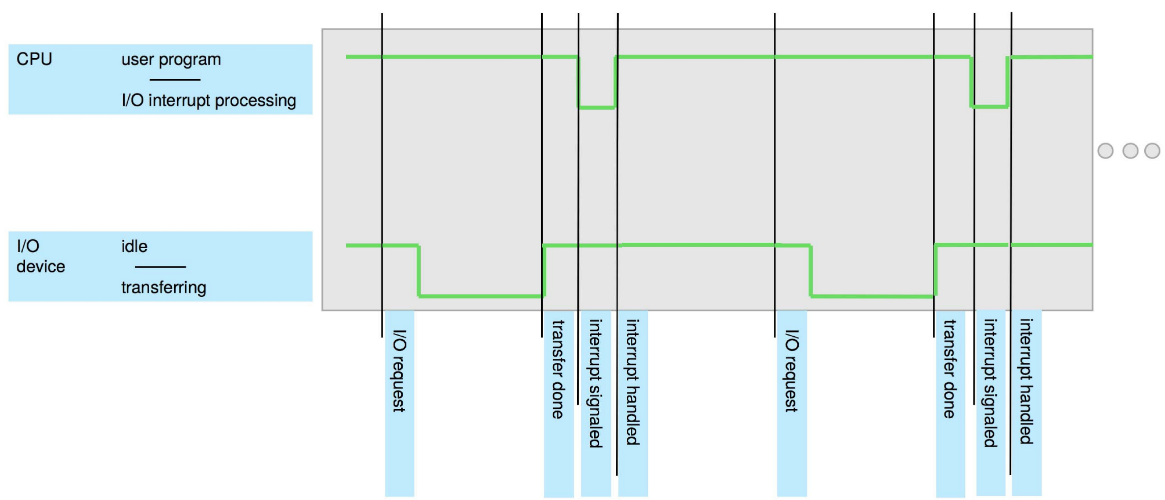
\includegraphics[width=0.8\textwidth]{images/interrupt_timeline.png}
    \caption{Intrrupt Timeline}
    \label{fig:Interrupt Timeline}
\end{figure}

\begin{figure}[H]
    \centering
    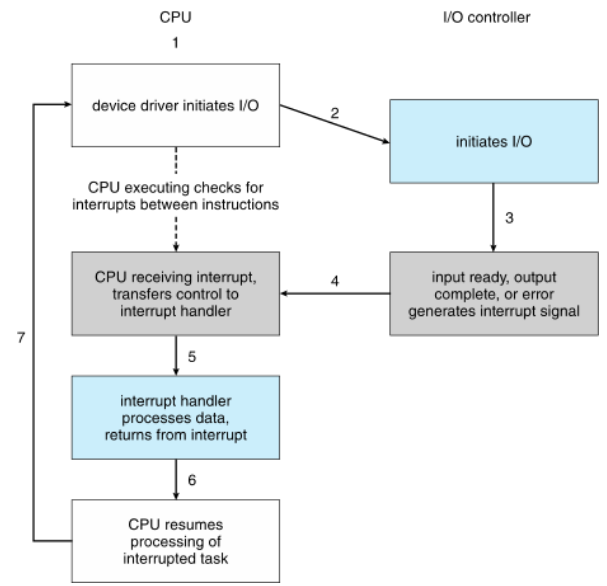
\includegraphics[width=0.5\textwidth]{images/Interrupt-drive_IO _Cycle.png}
    \caption{Interrupt-drive I/O Cycle}
    \label{fig:Interrupt-drive I/O Cycle}
\end{figure}


    \subsection{Input/Output Handling Methods}

    Operating systems employ two fundamentally different approaches for managing input/output operations, each with distinct advantages and trade-offs in terms of system efficiency and complexity.


    \subsubsection{Synchronous I/O Processing}

    The first method implements synchronous I/O processing, where the system maintains strict sequential control over input/output operations. When an I/O operation begins, the user program that initiated the request is immediately suspended and cannot continue execution until that specific I/O operation completes entirely. During this waiting period, the CPU executes a special wait instruction that effectively idles the processor until the next interrupt signals the completion of the I/O operation.
    This approach often involves the CPU in what is called a wait loop, where the processor repeatedly checks for the completion of the I/O operation. This creates contention for memory access, as the CPU continuously uses memory cycles to poll for status updates rather than performing useful work. The synchronous method enforces a strict limitation that only one I/O request can be outstanding at any given time, completely preventing simultaneous I/O processing across multiple devices. While this approach simplifies system design and ensures predictable behavior, it significantly underutilizes system resources and can lead to poor overall performance.


    \subsubsection{Asynchronous I/O Processing}

    The second method implements asynchronous I/O processing, which allows for much more efficient system resource utilization. Under this approach, when an I/O operation starts, control immediately returns to the user program without waiting for the I/O operation to complete. This allows the user program to continue executing other instructions while the I/O operation proceeds independently in the background.
    The operating system manages this complexity through a sophisticated system call mechanism that allows user programs to explicitly request when they need to wait for I/O completion. The OS maintains a comprehensive device-status table that contains detailed entries for each I/O device in the system. Each table entry includes critical information such as the device type, memory address, and current operational state.
    When managing asynchronous I/O operations, the operating system uses this device table as an index to quickly determine the status of any device and to modify table entries when interrupts occur. This allows the system to track multiple concurrent I/O operations across different devices while maintaining accurate state information. The asynchronous approach enables true parallelism between CPU operations and I/O activities, significantly improving overall system throughput and responsiveness.


    \subsection{Computer System Startup Process}

    The initialization of a computer system follows a carefully orchestrated sequence that transforms the hardware from a powered-off state into a fully functional computing environment running an operating system.


    \subsubsection{Bootstrap Program Execution}

    When a computer is first powered on or undergoes a reboot, the very first code that executes is called the bootstrap program, also known as the bootloader. This critical piece of software is permanently stored in non-volatile memory, typically in Read-Only Memory (ROM) or Erasable Programmable Read-Only Memory (EPROM). Because this code is stored in firmware that persists even when power is removed, it remains available immediately when the system starts up.
    The bootstrap program has the comprehensive responsibility of initializing all aspects of the computer system. This includes performing power-on self-tests to verify that critical hardware components are functioning properly, initializing memory controllers and other system chipsets, detecting and configuring attached devices, and establishing the basic hardware environment needed for more complex software to operate.


    \subsubsection{Operating System Loading}

    Once the bootstrap program has successfully initialized the hardware environment, its final and most important task is to locate, load, and start the execution of the operating system kernel. The kernel represents the core of the operating system and contains the fundamental code needed to manage system resources, handle hardware interactions, and provide services to application programs.
    The bootstrap process typically involves reading the kernel from a storage device such as a hard drive or solid-state drive into the computer's main memory, and then transferring control to the kernel's entry point. At this moment, the operating system begins its own initialization sequence, taking over system management from the simple bootstrap program and establishing the full computing environment that users and applications expect.


\section{Storage Structure}

    Let us look at the various types of stroage available, their characteristics and how they are organized in a computer system.
    The principal type are:
        \begin{itemize}
            \item \textbf{Main Memory:} This is the primary storage area that the CPU directly accesses to read and write data. It is typically volatile, meaning that its contents are lost when power is turned off. Main memory is fast but limited in size compared to secondary storage.
            \item \textbf{Secondary Storage:} This includes devices like hard drives, solid-state drives, and optical discs. Secondary storage is non-volatile, meaning it retains data even when the computer is powered down. It provides much larger storage capacity than main memory but is slower to access. Is important note that secondary storage is not directly accessible by the CPU; data must first be loaded into main memory.
            \item \textbf{Hard Disk Drives (DD):} This is typically a rigid metal or glass platters covered with magnetic recording material. Data is stored in concentric tracks, which are divided into sectors. The disk controller determines the logiacl interation between the device and the compuyer.
            \item \textbf{Non-Volatile Memory (NVM):} This includes technologies like flash memory and solid-state drives (SSDs). NVM retains data without power and offers faster access times compared to traditional hard drives. It is commonly used in portable devices and as a faster alternative to HDDs in computers. 
        \end{itemize}
    
    Let us define two important concepts:
        \begin{itemize}
            \item \textbf{Caching:} copying information into faster storage system; main memory can be viewed as a cache for secondary storage.
            \item  \textbf{Device Driver:} for each device controller to manage I/O. Provides uniform interface between controller and kernel.
        \end{itemize}



\begin{figure}[H]
    \centering
    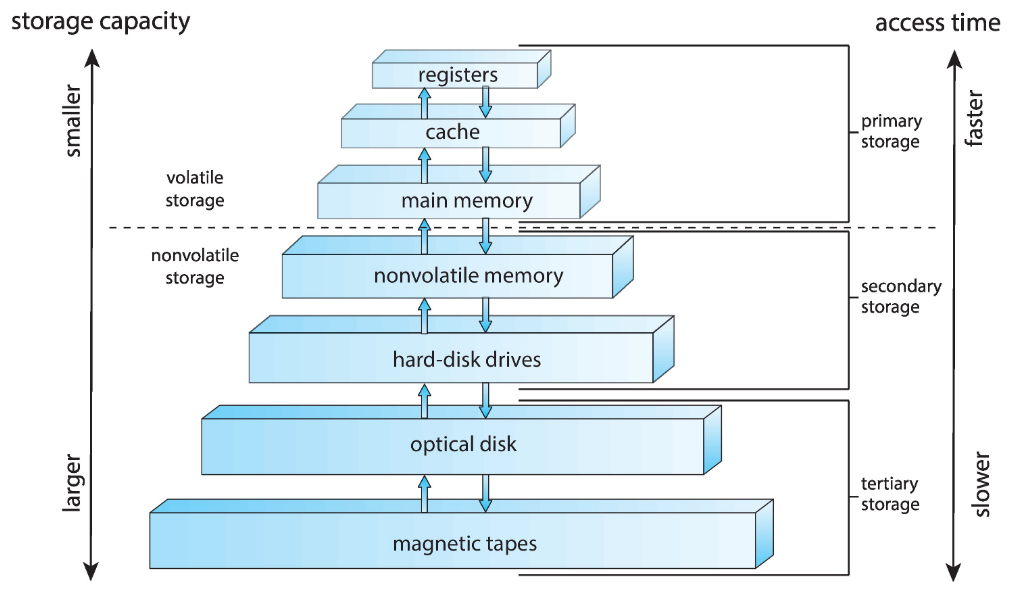
\includegraphics[width=0.6\textwidth]{images/storage_hieracacy.png}
    \caption{Storage Hierarchy}
    \label{fig:storage_hierarchy}
\end{figure}

\noindent
\begin{minipage}[t]{0.45\textwidth}
    \textbf{Direct Memory Access (DMA)} is a hardware controller that allows certain devices to transfer data directly to or from main memory without continuous involvement of the CPU. Without a DMA controller, the CPU would need to handle every step of the data transfer, significantly slowing down the system. With DMA, the CPU can perform other tasks while the transfer occurs in the background.
\end{minipage}
\hfill
\begin{minipage}[t]{0.5\textwidth}
    \vspace{0.5cm} % Aggiusta lo spazio verticale per allineare meglio l'immagine
    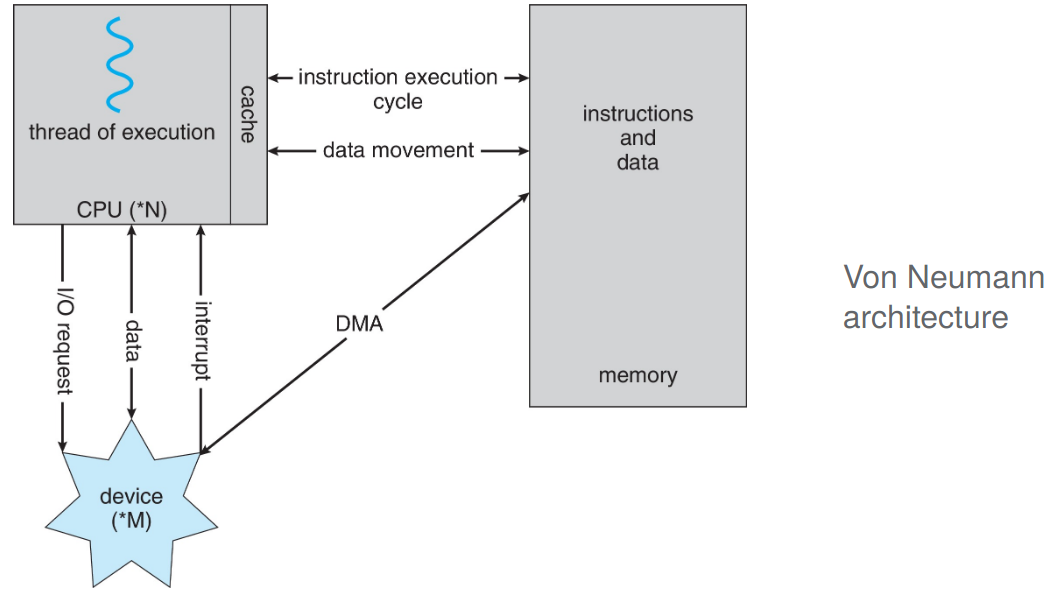
\includegraphics[width=\textwidth]{images/computer_works2.png}
    \captionof{figure}{How computers work}
    \label{fig:computer_works}
\end{minipage}

    \subsection{Multiprogramming Systems}

The evolution of computing systems revealed a fundamental inefficiency in single-program execution environments. When a computer system runs only one program at a time, a single user cannot consistently maintain full utilization of both the CPU and input/output devices. This occurs because programs frequently require different types of resources at different times, leading to periods where expensive hardware components remain idle while waiting for other operations to complete.
Multiprogramming addresses this inefficiency by organizing multiple jobs, each consisting of both executable code and associated data, in such a way that the CPU always has at least one job available for execution. The operating system maintains a subset of the total jobs in the system within main memory, creating a pool of ready-to-execute programs. Through a process called job scheduling, the operating system intelligently selects which job should run at any given moment.
The key advantage of multiprogramming becomes apparent when a currently executing job encounters a situation requiring it to wait, such as when it needs to perform input/output operations. Rather than allowing the CPU to remain idle during these waiting periods, the operating system immediately switches execution to another job that is ready to run. This context switching ensures continuous CPU utilization and dramatically improves overall system throughput by overlapping the execution of multiple programs.


    \subsection{Multitasking and Timesharing Systems}

Multitasking represents a logical extension of batch multiprogramming systems, introducing the concept of interactive computing through rapid job switching. In a multitasking environment, the CPU switches between jobs so frequently that users can actively interact with each job while it appears to be running continuously. This creates the illusion of simultaneous execution across multiple programs, even on systems with a single processor.
The effectiveness of multitasking systems depends critically on maintaining responsive interaction with users. Response times must typically remain under one second to preserve the interactive experience that users expect. Each user in the system has at least one program executing in memory, and these executing programs are referred to as processes to distinguish them from the static job concept used in batch systems.
When multiple processes are simultaneously ready to run, the operating system must employ CPU scheduling algorithms to determine which process should receive processor time and for how long. These scheduling decisions directly impact system responsiveness and fairness among competing processes.
Memory management presents additional challenges in multitasking systems. When the total memory requirements of all active processes exceed the available physical memory, the operating system employs a technique called swapping, which moves entire processes between main memory and secondary storage as needed. This allows more processes to participate in multitasking than could otherwise fit simultaneously in memory.
Virtual memory systems provide an even more sophisticated solution by allowing the execution of processes that are not completely loaded into main memory. Through virtual memory mechanisms, portions of a process can reside on secondary storage while other portions remain in main memory, creating the illusion of a much larger memory space than physically available.


    \subsection{Dual-Mode Operation and System Protection}

    Modern operating systems implement dual-mode operation as a fundamental security mechanism that allows the OS to protect itself and other critical system components from potentially harmful user programs. This protection scheme establishes two distinct execution modes that define what operations and resources are available to currently executing code.


    \subsubsection{User Mode and Kernel Mode}

    The dual-mode system distinguishes between user mode and kernel mode execution environments. User mode provides a restricted execution environment where application programs run with limited access to system resources and hardware components. In contrast, kernel mode grants unrestricted access to all system resources, hardware devices, and critical system operations.
The hardware provides direct support for this dual-mode operation through a special mode bit that indicates the current execution mode of the processor. When user application code is executing, the mode bit is set to indicate user mode, automatically enforcing the associated restrictions. When the operating system kernel code is executing, the mode bit indicates kernel mode, granting full system access.



\subsubsection{Mode Transition and System Calls}

    The transition between user mode and kernel mode occurs through a carefully controlled mechanism that prevents user programs from arbitrarily elevating their privileges. Users cannot directly manipulate the mode bit to gain kernel-level access, as this would completely undermine system security.
    Instead, mode transitions occur through system calls, which provide a controlled interface for user programs to request operating system services. When a user program makes a system call, the hardware automatically changes the mode bit to kernel mode, allowing the operating system to perform the requested operation with full system privileges. Upon completion of the system call, the mode bit is automatically reset to user mode before returning control to the user program.



\begin{figure}[H]
    \centering
    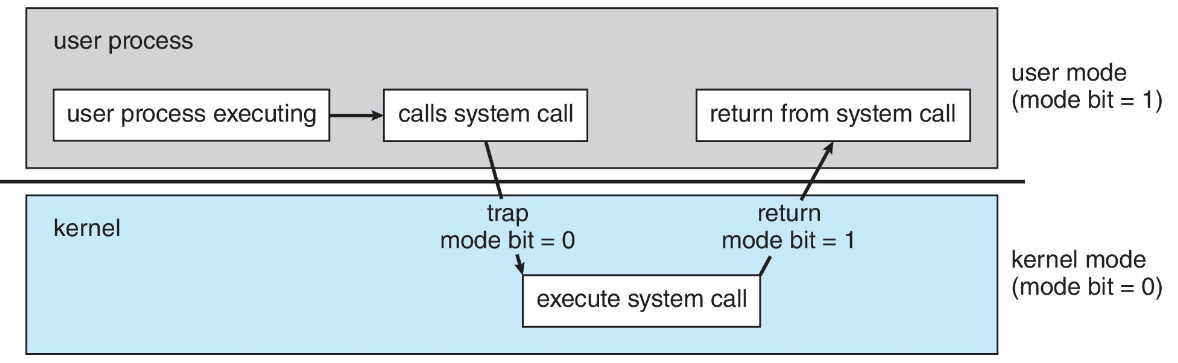
\includegraphics[width=0.6\textwidth]{images/user_kernel.png}
    \caption{User Kernel transition}
    \label{fig:User_Kernel transition}
\end{figure}

\subsubsection{Privileged Instructions}

The dual-mode system designates certain critical instructions as privileged, meaning they can only be executed when the processor is operating in kernel mode. These privileged instructions typically involve operations that could compromise system security or stability if misused, such as direct hardware manipulation, memory management operations, or modification of critical system data structures.
When user mode code attempts to execute a privileged instruction, the hardware generates an exception that transfers control to the operating system kernel. The kernel can then determine whether the attempted operation should be permitted and either perform it on behalf of the user program or terminate the program if the operation represents a security violation.



\subsection{Timer-Based Process Control}

Operating systems require mechanisms to prevent individual processes from \textbf{monopolizing system resources} or executing indefinitely in ways that could harm overall system performance. The \textbf{timer mechanism} provides a fundamental solution to prevent \textbf{infinite loops} and processes from hogging system resources through \textbf{hardware-enforced time limits}.
The timer system operates through a \textbf{hardware counter} that is continuously \textbf{decremented by the physical system clock}. This counter serves as a countdown mechanism that automatically \textbf{generates an interrupt when it reaches zero}, regardless of what code is currently executing. The operating system, executing in kernel mode with \textbf{privileged instructions}, has \textbf{exclusive control over setting this counter value}, preventing user programs from manipulating the timer to avoid time limits.
Before scheduling any process to run, the operating system configures the timer by setting the counter to an appropriate value that represents the \textbf{maximum time slice} allocated to that process. This proactive setup ensures that the operating system will \textbf{regain control} either when the process voluntarily relinquishes the CPU or when the \textbf{timer expires}. If a process exceeds its allotted time, the \textbf{timer interrupt} allows the operating system to forcibly terminate or suspend the offending program, maintaining \textbf{system responsiveness and fairness} among competing processes.


\subsection{Process Management}

Process management represents one of the most critical responsibilities of modern operating systems, encompassing the \textbf{creation, execution, and termination} of programs throughout their lifecycle.


\subsubsection{Process Definition and Characteristics}

A \textbf{process} fundamentally differs from a \textbf{program} in that it represents a \textbf{program in active execution} rather than a static collection of instructions. While a program exists as a \textbf{passive entity} stored on disk, a process becomes an \textbf{active entity} that consumes system resources and performs computational work within the system environment.
Every process requires access to various \textbf{system resources} to accomplish its designated tasks. These resources include \textbf{CPU time} for instruction execution, \textbf{memory space} for storing both instructions and data, \textbf{input/output capabilities} for interacting with external devices, access to \textbf{files} for persistent data storage, and \textbf{initialization data} needed to establish the process's starting state. When a process terminates, the operating system \textbf{reclaims these reusable resources}, making them available for other processes.


\subsubsection{Single-Threaded and Multi-Threaded Processes}

Traditional \textbf{single-threaded processes} maintain a \textbf{single program counter} that specifies the location of the next instruction to execute. These processes follow a \textbf{strictly sequential execution model}, executing one instruction after another until completion. This straightforward approach simplifies process management but limits the potential for parallelism within individual programs.
\textbf{Multi-threaded processes} extend this model by maintaining \textbf{multiple program counters}, with each thread of execution having its own counter. This allows a single process to pursue \textbf{multiple concurrent lines of execution}, potentially improving performance through parallelism and better resource utilization.
Modern computer systems typically manage many processes simultaneously, including both \textbf{user applications} and \textbf{operating system processes}, running concurrently across one or more CPUs. The operating system achieves this \textbf{concurrency through multiplexing}, rapidly switching CPU time among the various processes and threads to create the illusion of simultaneous execution.


\subsubsection{Operating System Process Management Activities}

The operating system maintains comprehensive control over process lifecycle management through several key activities. It handles the \textbf{creation and deletion} of both user processes and system processes, managing the allocation of resources and the cleanup of terminated processes. The system provides mechanisms for \textbf{suspending and resuming processes}, allowing for sophisticated scheduling and resource management strategies.
\textbf{Process synchronization mechanisms} ensure that multiple processes can coordinate their activities and share resources safely without interfering with each other. \textbf{Process communication facilities} enable processes to exchange data and coordinate their actions. Additionally, the operating system implements \textbf{deadlock handling mechanisms} to detect and resolve situations where processes become stuck waiting for each other in circular dependency chains.


\subsection{Memory Management}

Effective memory management stands as a cornerstone of operating system functionality, directly impacting both \textbf{system performance} and \textbf{user experience} through its influence on program execution and resource utilization.


\subsubsection{Memory Requirements for Program Execution}

For any program to execute successfully, \textbf{all or part of its instructions must reside in main memory} where the CPU can access them directly. Similarly, the \textbf{data required by the program must also be available in memory} during execution. This fundamental requirement drives the need for sophisticated memory management systems that can optimize the use of \textbf{limited physical memory resources}.
Memory management systems determine \textbf{what information resides in memory at any given time}, making strategic decisions about which programs and data should be kept readily accessible. These decisions directly impact \textbf{CPU utilization and computer response times}, as programs cannot execute efficiently if their required instructions or data are not available in memory.


\subsubsection{Memory Management Activities}

The operating system performs several critical memory management activities to ensure efficient system operation. It continuously \textbf{tracks which parts of memory are currently in use} and identifies which processes or system components are using specific memory regions. This tracking enables the system to make informed decisions about \textbf{memory allocation and deallocation}.
The system must decide \textbf{which processes or portions of processes should be moved into and out of memory} based on current system demands and available resources. \textbf{Memory allocation and deallocation operations} must be performed dynamically as processes are created, grow, shrink, and terminate, ensuring that memory resources are used efficiently and that processes receive the memory they need to function properly.


\subsection{File System Management}

File system management provides users and applications with a \textbf{uniform, logical view of information storage} that abstracts away the complexities and variations of physical storage devices.


\subsubsection{File Abstraction and Storage Media}

The file system creates a \textbf{logical storage abstraction called a file}, which hides the physical properties and limitations of underlying storage media. Different storage devices, such as \textbf{disk drives} and \textbf{tape drives}, have vastly different characteristics including \textbf{access speed}, \textbf{storage capacity}, \textbf{data transfer rates}, and \textbf{access methods} that may be either sequential or random. The \textbf{file system abstraction} allows applications to work with files uniformly regardless of these underlying physical differences.


\subsubsection{File System Organization and Management}

Files are typically organized into \textbf{hierarchical directory structures} that provide logical organization and easier navigation of stored information. Most systems implement \textbf{access control mechanisms} that determine which users or processes can access specific files and what types of operations they can perform.
The operating system handles fundamental file operations including \textbf{creating and deleting both files and directories}. It provides \textbf{primitive operations for manipulating files and directories}, such as reading, writing, copying, and moving. The system manages the \textbf{mapping of logical files onto physical secondary storage} devices, handling the complex task of translating file operations into appropriate storage device operations.
Additionally, file systems implement \textbf{backup mechanisms} to copy important files onto \textbf{stable, non-volatile storage media}, protecting against data loss from hardware failures or other system problems.


\subsection{Mass Storage Management}

Mass storage management addresses the critical need for managing \textbf{large-capacity storage devices} that hold data not fitting in main memory or requiring \textbf{long-term persistence}.


\subsubsection{Importance of Mass Storage}

\textbf{Disk storage systems} typically serve as the primary repository for data that exceeds main memory capacity or must be preserved for extended periods. The performance characteristics of the \textbf{mass storage subsystem} and its associated \textbf{management algorithms significantly influence overall computer system speed}, making proper storage management critically important for system performance.


\subsubsection{Mass Storage Management Activities}

The operating system performs numerous activities related to mass storage management. \textbf{Mounting and unmounting operations} make storage devices available to the system and safely disconnect them when no longer needed. \textbf{Free space management} tracks available storage space and allocates it to files as needed.
\textbf{Storage allocation algorithms} determine how files are physically stored on storage devices, impacting both performance and space utilization. \textbf{Disk scheduling algorithms} optimize the order in which storage requests are processed to minimize access times and improve overall throughput.
\textbf{Partitioning} allows storage devices to be divided into separate logical units, each potentially using different file systems or serving different purposes. \textbf{Protection mechanisms} ensure that stored data remains secure and that unauthorized access attempts are prevented, maintaining \textbf{data integrity and system security}.


\subsection{Caching}

    The caching principle is implemented at multiple levels in a computer system: in hardware, the operating system, and software. The main idea is to keep a copy of frequently accessed information in a faster storage layer. The cache is smaller than the original storage and is checked first. If the requested information is found (cache hit), it is used directly. If not (cache miss), it is fetched from the original storage and a copy is placed in the cache.
    Caching is a generic concept: for example, L1 cache is a cache for L2 cache, main memory acts as a cache for secondary storage, and so on.
    The main challenge with caching is \textbf{consistency} between the cache and the original storage. When data in the original storage is updated, the corresponding cache entries must also be updated or invalidated to avoid stale data. This process is typically managed by hardware mechanisms and cache coherence protocols.



\begin{figure}[H]
    \centering
    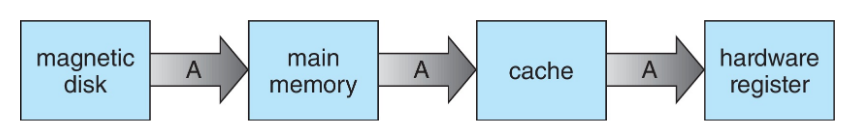
\includegraphics[width=0.6\textwidth]{images/migration_data.png}
    \caption{Migration data A}
    \label{fig: MIgration data A}
\end{figure}

\subsection{I/O Subsystem}

    The I/O subsystem of an operating system serves to abstract the complexities of hardware devices from the user, providing a consistent interface regardless of the underlying device. It manages memory associated with I/O operations, including buffering, caching, and spooling. Buffering temporarily stores data while it is being transferred between devices or memory, improving efficiency. Caching stores frequently accessed portions of data in faster storage to enhance performance. Spooling allows data to be stored temporarily, often to coordinate the use of slower devices, such as printers. The subsystem also provides a general device-driver interface and includes drivers for specific hardware, enabling the OS to communicate effectively with a wide variety of devices.


\subsection{Protection and Security}

    Protection mechanisms in an operating system control which processes or users can access system resources, while security mechanisms defend the system from both internal and external threats. Security concerns include threats such as viruses, worms, identity theft, and denial-of-service attacks. Operating systems generally manage security by identifying users through user IDs and associating those IDs with files, processes, and privileges. Group IDs allow administrators to manage access for sets of users efficiently. Additionally, some systems implement privilege escalation, which allows a user to temporarily assume an identity with higher rights to perform specific tasks while maintaining overall system security.


\subsection{Virtualization}

Virtualization enables operating systems to run applications or even entire guest operating systems on top of a host OS, providing a flexible and isolated execution environment. It is commonly used to run software compiled for different CPU architectures, in which case \textbf{emulation} may be employed, although it is typically slower. Native virtualization allows guest OSes to run directly on the host CPU, managed by a Virtual Machine Manager (VMM) or hypervisor, which handles resource allocation and isolation. Virtualization is widely used for testing applications across multiple OSes, running multiple OS environments on a single machine, or managing virtualized compute resources in data centers. Some VMMs, like VMware ESX or Citrix XenServer, run directly on hardware without a conventional host OS, providing high-performance virtualization at scale.



\begin{figure}[H]
    \centering
    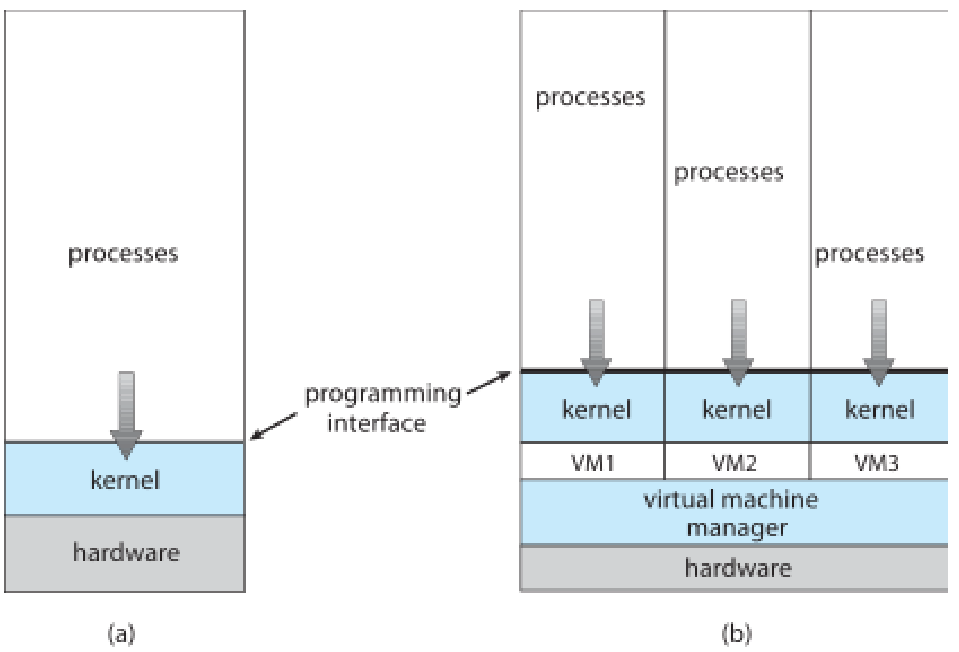
\includegraphics[width=0.5\textwidth]{images/Screenshot from 2025-09-16 16-10-00.png}
    \caption{VM envorionment}
    \label{fig: VM envorionment}
\end{figure}

\section{Computer System Architecture}

\subsection{Multiprocessor Systems}
Multiprocessor systems are widely used because they increase throughput, reduce costs by sharing resources, and improve reliability through graceful degradation, meaning that the system can continue working even if one processor fails. In some cases, these systems combine general-purpose and special-purpose processors to achieve higher efficiency.  
The organization of multiprocessor systems can be described in two main models:
\begin{itemize}
    \item \textbf{Asymmetric multiprocessing:} each processor is assigned a specific task.
    \item \textbf{Symmetric multiprocessing:} all processors perform the same tasks and share the workload.
\end{itemize}

\begin{figure}[H]
    \centering
    \begin{minipage}{0.4\textwidth}
        \centering
        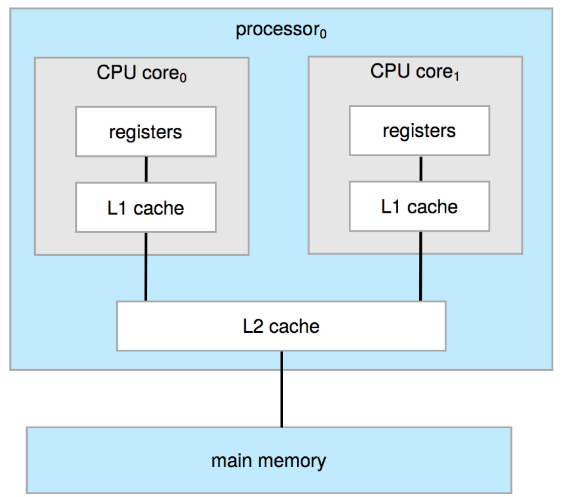
\includegraphics[width=\textwidth]{images/Dual_Core_Design.png}
        \caption{Dual Core Design}
        \label{fig:Dual_Core_Design}
    \end{minipage}
    \hfill
    \begin{minipage}{0.4\textwidth}
        \centering
        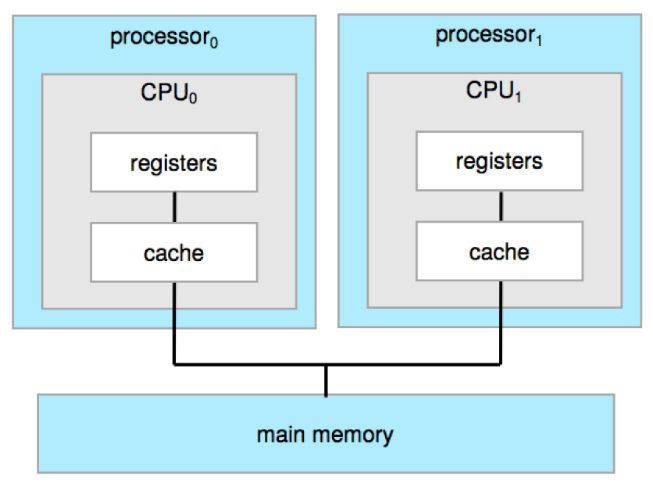
\includegraphics[width=\textwidth]{images/Symmetric _Multiprocessing_Architecture.png}
        \caption{Symmetric Multiprocessing Architecture}
        \label{fig:Symmetric_Multiprocessing_Architecture}
    \end{minipage}
    \label{fig:dual_vs_symmetric}
\end{figure}

\subsection{Clustered Systems}
Clustered systems connect multiple independent computers that cooperate as a single unit, often sharing storage through a storage-area network. Their main goal is to provide high availability, allowing services to survive hardware failures, but they can also be designed for high-performance computing, where applications must be parallelized. To avoid conflicting operations on shared resources, some clusters employ distributed lock managers.  
Clustered systems are typically organized in two main ways:
\begin{itemize}
    \item \textbf{Asymmetric clustering:} one machine remains in standby mode and takes over if another system fails.
    \item \textbf{Symmetric clustering:} all nodes are active, running applications and monitoring each other.
\end{itemize}


\begin{figure}[H]
    \centering
    \begin{minipage}{0.4\textwidth}
        \centering
        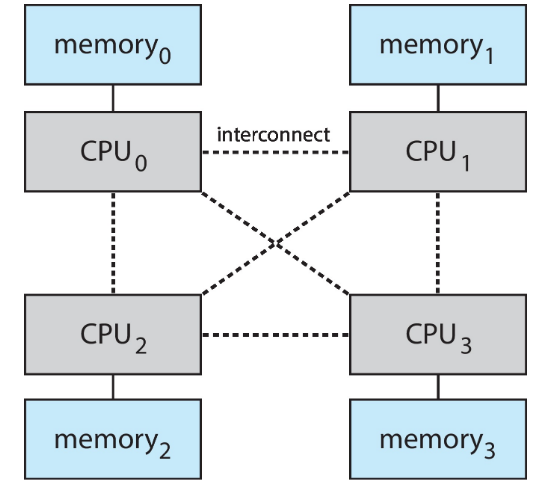
\includegraphics[width=\textwidth]{images/NUMA.png}
        \caption{NUMA Architecture}
        \label{fig:NUMA Architecture}
    \end{minipage}
    \hfill
    \begin{minipage}{0.5\textwidth}
        \centering
        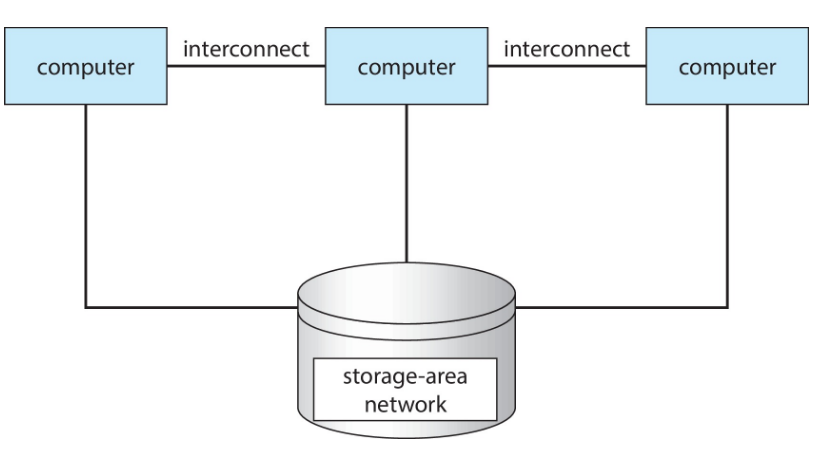
\includegraphics[width=\textwidth]{images/Clustered_System.png}
        \caption{Clustered System Architecture}
        \label{fig:Clustered System Architecture}
    \end{minipage}
    \label{fig:dual_vs_symmetric}
\end{figure}